\question{4.17}{Een conservatoriumstudent oefent per dag tussen 180 en 300 minuten. Het aantal oefenuren op een willekeurige dag kan worden weergegeven
door een continue kansvariabele $X$ (in uren) met de volgende kansdichtheid:
\[
    f(x) = \begin{cases} 0,40, & \text{ voor } 3,00 \le x < 4,00 \\ 0,60, & \text { voor } 4,00 \le x < 5,00 \\ 0, & \text{ elders.} \end{cases}\\
\]
}
\begin{enumerate}[label=(\alph*)]
    \item Geef de kansdichtheid grafisch weer.
    \answer{
        \begin{center}
            \resizebox{0.9\textwidth}{!}{
                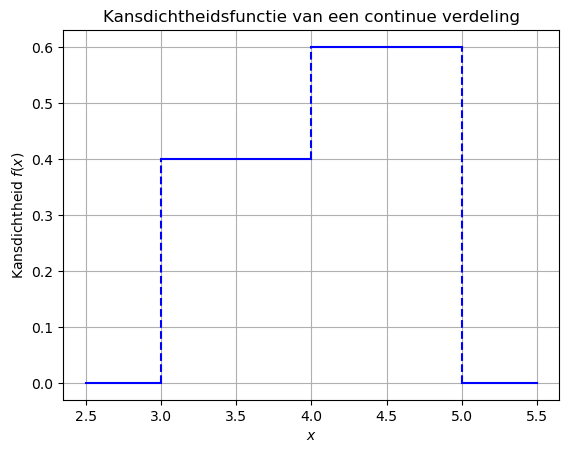
\includegraphics{opg4.17a.png}
            }
        \end{center}
    }
    
    \item Hoe groot is de kans dat de student op een willekeurige dag minder dan 210 minuten oefent? Hoe groot is de kans dat hij tussen 200 en 260 minuten oefent?
    \answer{
        De kans dat een student op een willekeurige dag minder dan 210 minuten, oftewel 3,5 uur oefent, is gelijk aan
        \[
            P(X \le 3,5) = \int_{-\infty}^{3,5} f(x) dx = \int_{3,00}^{3,5} 0,40 dx = \textrm{fnInt}(0.40; X; 3.00; 3.5) = 0,2.
        \]
        De kans dat een student op een willekeurige dag tussen 200 en 260 minuten oefent, oftewel tussen $\frac{10}{3}$ en $\frac{13}{3}$ uur oefent, is gelijk aan
        \begin{align*}
            P(\frac{10}{3} \le X \le \frac{13}{3}) &= \int_{\frac{10}{3}}^{\frac{13}{3}} f(x)\ dx \\
                                                   &= \int_{\frac{10}{3}}^{4,00} 0,40\ dx + \int_{4,00}^{\frac{13}{3}} 0,6\ dx \\
                                                   &= \textrm{fnInt}(0.40; X; 10/3; 4.00) + \textrm{fnInt}(0.60; X; 4.00; 13/3) \\
                                                   &\approx 0,4667
        \end{align*}
    }
    
    \item Wat is de verwachtingswaarde van de dagelijkse studietijd?
    \answer{
        De verwachtingswaarde van de dagelijkse studietijd berekenen we met de algemene formule voor continue kansverdelingen:
        \begin{align*}
            E[X]    &= \int_{-\infty}^{\infty} x \cdot f(x)\ dx \\
                    &= \int_{3,00}^{4,00} x \cdot 0,40\ dx + \int_{4,00}^{5,00} x \cdot 0,60\ dx \\
                    &= \textrm{fnInt}(0.40X; X; 3.00; 4.00) + \textrm{fnInt}(0.60X; X; 4.00; 5.00) \\
                    &= 4,1
        \end{align*}
        De verwachte dagelijkse studietijd is 4,1 uur, oftewel 246 minuten.
    }
\end{enumerate}